\begin{frame}{Learning}
    \framesubtitle{Knowledge Acquisition}
    \begin{itemize}
        \item A natural follow-up question after categorizing knowledge is to ask: ``How do we, or any other \emph{intelligent} entity, obtain knowledge?''
        \item We call the process of knowledge-acquisiton \bhighlight{learning}.
        \item We'll discuss three beliefs that played critical roles in the formative years of AI, which will hopefully demystify the direction AI research has taken during the last few decades.
    \end{itemize}
\end{frame}

% Symbolism
\begin{frame}{Symbolism}
    \framesubtitle{The Symbolic Paradigm}
    \begin{itemize}
        \item The core idea within \bhighlight{symbolism} is that knowledge lives in discrete chunks called \bhighlight{symbols} and the mind is a ``symbol processing machine''. \\
        \item Symbolists posit the existence of a mental \bhighlight{language} akin to natural human language, where thoughts are formed via \bhighlight{logical} ($\land$, $\lor$, $\neg$, $\implies$) combinations
              of the \emph{words} within this language.
        \item In this view, the mind is much like a machine processing a list of instructions.
    \end{itemize}
\end{frame}

\begin{frame}{Symbolism}
    \framesubtitle{Symbolic Reasoning Diagram}
    \begin{figure}
        \centering
        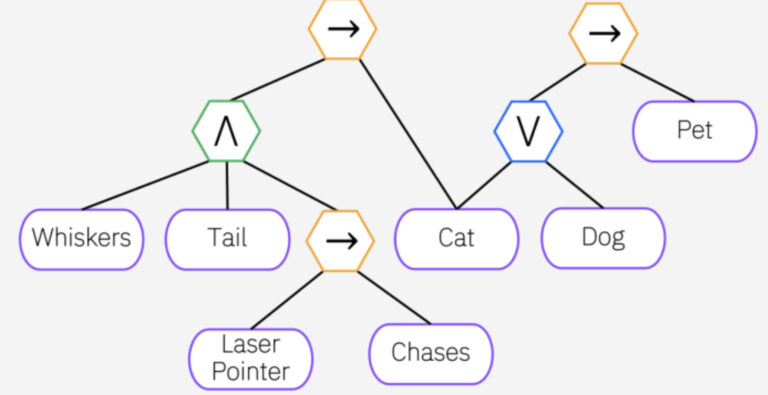
\includegraphics[width=0.8\linewidth]{images/symbolic-ai.jpg}
        \caption{A simplified logical decomposition of a thought. \gcite{\href{https://startupkitchen.community/neuro-symbolic-ai-why-is-it-the-future-of-artificial-intelligence/}{Source}}}
    \end{figure}
\end{frame}

\begin{frame}{Symbolism}
    \framesubtitle{History}
    \begin{itemize}
        \item This view dominated the field of AI between the mid-1950s and the mid-1990s.
        \item Classical AI such as \bhighlight{decision trees} or \bhighlight{rule-based systems} followed this philosophy.
        \item Such systems are now dubbed \bhighlight{GOFAI} (good old-fashioned artificial intelligence).
        \item A key feature of these systems was their \bhighlight{transparent} decision making, a feature somewhat lost in modern approaches such as neural networks,
              which has led to a resurgence of symbolic AI in hybrid approaches called \bhighlight{neuro-symbolic} AI.
    \end{itemize}
\end{frame}

% Associationism
\begin{frame}{Associationism}
    \framesubtitle{Linking Ideas through Experience}
    \begin{itemize}
        \item Historically preceding symbolism yet paramount to subsequent theories of intelligence, \bhighlight{associationism} states that minds form knowledge by linking ideas through experience.
        \item One of the most foundational works in explaining how neurons learn is the theory of \bhighlight{Hebbian learning}, which applies the associative principle of learning to the brain:
              ``neurons that fire together wire together.''
    \end{itemize}
\end{frame}

\begin{frame}{Associationism}
    \framesubtitle{Principles of Associative Learning}
    The classical ``laws'' of association are as follows:
    \begin{itemize}
        \item \textbf{Contiguity:} Things that occur together in time or space become linked (e.g., lightning and thunder).
        \item \textbf{Similarity:} Things that share features become linked (e.g., thinking of an apple might make you think of a pear).
        \item \textbf{Contrast:} Opposites become linked (e.g., thinking of hot brings up cold).
        \item \textbf{Repetition:} Things paired often become strongly linked (e.g., hearing a song every morning ties it to waking up).
    \end{itemize}
\end{frame}

\begin{frame}{Associationism}
    \framesubtitle{Pavlov’s Conditioning}
    A famous example of associative learning is \bhighlight{Pavlov's dog} experiment, which explores classical conditioning:
    \begin{figure}
        \centering
        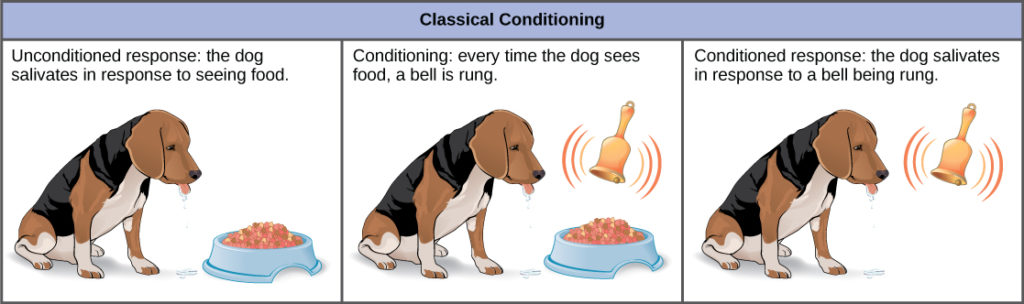
\includegraphics[width=\linewidth]{images/pavlov-dog.jpg}
        \caption{Pavlov's experiment. \gcite{\href{https://courses.lumenlearning.com/wm-biology2/chapter/learned-behaviors/}{Source}}}
    \end{figure}
\end{frame}

% Connectionism
\begin{frame}{Connectionism}
    \framesubtitle{Distributed Representations}
    \begin{itemize}
        \item \bhighlight{Connectionism} posits that knowledge arises from networks of interconnected, simple processing units inspired by neural structures in biological brains.
        \item Unlike symbolism, connectionism does not rely on explicit symbolic representations but rather on distributed representations across many units (neurons).
        \item Knowledge is represented implicitly in the \bhighlight{connections} between units and the \bhighlight{strengths (weights)} of these connections.
    \end{itemize}
\end{frame}

\begin{frame}{Connectionism}
    \framesubtitle{Training Connectionist Networks}
    \begin{itemize}
        \item Connectionism emphasizes \bhighlight{parallel distributed processing (PDP)}—many interconnected processing elements working simultaneously.
        \item Learning in connectionism occurs by adjusting the connection strengths (weights) based on experience, a process called \bhighlight{training}.
        \item Connectionist training often uses \bhighlight{gradient-based learning}, where weights are nudged little by little in the direction that reduces error, and an \bhighlight{expectation–maximization (EM)} style approach, which alternates between guessing how each part of the network contributes to the task and then updating the weights to improve performance.
    \end{itemize}
\end{frame}

\begin{frame}{Connectionism}
    \framesubtitle{Structure of an Artificial Neural Network}
    \begin{figure}
        \centering
        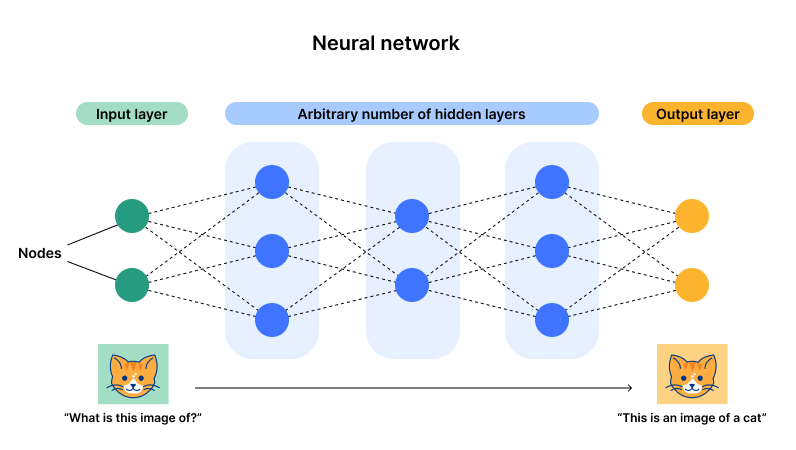
\includegraphics[width=\linewidth]{images/neural-network.png}
        \caption{An artificial neural network (ANN) composed of interconnected nodes, inspired by biological neural networks. \gcite{\href{https://www.cloudflare.com/learning/ai/what-is-neural-network/}{Source}}}
    \end{figure}
\end{frame}

\begin{frame}{Connectionism}
    \framesubtitle{Rise of Deep Learning}
    \begin{columns}[c]
        \begin{column}{0.6\linewidth}
            \begin{itemize}
                \item Connectionism rose to prominence in the 1980s and is the foundation for modern \bhighlight{deep learning}, the dominant approach in AI today.
                \item Models like \bhighlight{artificial neural networks} excel at pattern recognition and learning but their lack of interpretability drives ongoing research in explainable AI.
            \end{itemize}
        \end{column}
        %
        \begin{column}{0.4\linewidth}
            \begin{figure}
                \centering
                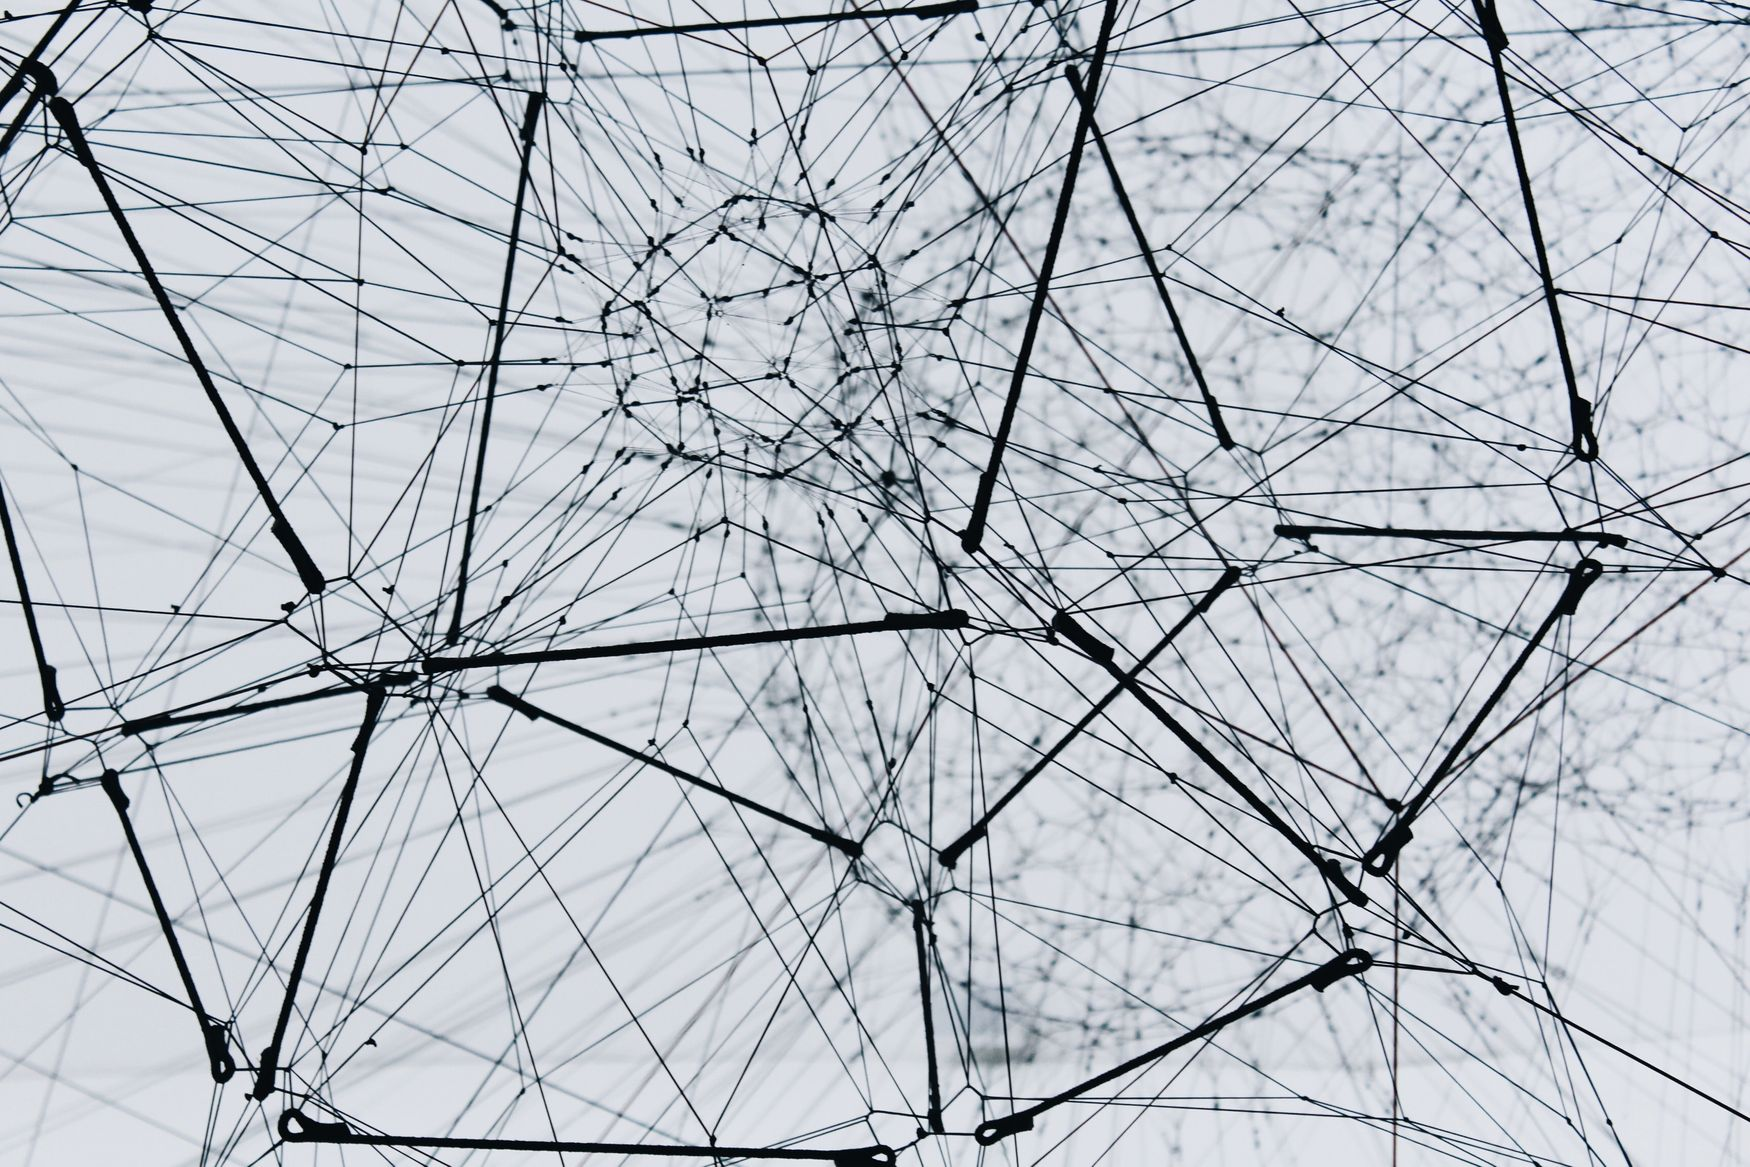
\includegraphics[width=\columnwidth]{images/connectionism.jpg}
                \caption{Photo of an interconnected metal structure, resembling connectionist machines. \gcite{\href{https://unsplash.com/photos/low-angle-photography-of-metal-structure-ZiQkhI7417A}{Source}}}
            \end{figure}
        \end{column}
    \end{columns}
\end{frame}